%Etude des solutions de réalisation technique possible
%Choix technologique retenus
%Justification de ces choix avec avantages et inconvénients


\subsection{Méthodes d'extraction du texte du document}
Afin d'analyser un document pdf, nous devons en premier lieu en extraire le texte brut, appelé ici \textit{transcript}.
L'extraction du transcript dépend de la manière dont le document a été enregistré: Souvent le texte est directement présent dans le document lui même, mais il arrive que le pdf soit stocké sous la forme d'une suite d'images (lorsque le document est un scan par exemple).

\subsubsection{Cas du pdf \textit{full text}}
Le format pdf contient normalement directement le transcript du document.
Dans ce cas, plusieurs programmes existent pour le récupérer: pdftotext, poppler, \ldots 
Nous avons choisi pdftotext car c'est l'outil open source le plus suivi et le plus utilisé, ce qui le rend très probable d'être déjà présent sur l'ordinateur exécutant le programme d'extraction.
De plus sa popularité le rend très probablement plus durable.

\subsubsection{Cas du pdf image}
Si le document pdf ne contient pas de texte récupérable par pdftotext, nous devons passer par des techniques d'OCR (Optical Character Recognition).
Ces techniques nous permettent d'extraire le texte d'une image grâce à des techniques avancées de machine learning.

Notre recherche pour l'état de l'art a relevé les techniques suivantes:
\begin{itemize}
\item \textbf{Tesseract}
État de l'art de l'OCR open source pour le moment (score d'environ 90\%)
\item \textbf{OCRupus}
Logiciel très réputé d'OCR (score d'environ 70\%)
\end{itemize}
Nous avons écarté l'idée de construire notre propre modèle au vu du temps très limité du projet.

Notre choix s'est porté sur l'état de l'art actuel, Tesseract, pour ses meilleures performances et le fait qu'une librairie python est disponible pour l'utiliser directement.

Les logiciels d'OCR peuvent être utilisés directement sur les documents pdf transformés en images (format TIF) mais les performances obtenues ne seront pas optimales.
Le document traité doit passer par une étape de traitement d'image, puis de nettoyage du texte obtenu, qui contient forcément des erreurs.

\subsection{Extraction des données d'importance}
Les données à récupérer dans le document peuvent être séparées en deux catégories: normées et non normées.

Les données normées (les références de RAA par exemple) respectent tout le temps les mêmes méthodes de notation et peuvent donc être récupérées par simple comparaison de texte, ce qui en fait une tache peu complexe.
Pour cela, on peut utiliser des RegEx qui sont des chaines de caractères normées permettant la recherche de termes similaires en forme.
Leur utilisation se rapproche d'une forme de programmation.

Les données non normées, comme les noms propres, sont un cas plus difficile car ils n'ont pas de format fixe.
Pour les trouver dans le texte, nous pouvons utiliser des systèmes de \gls{NLP} comme Spacy, qui possèdent des fonctions intégrées de reconnaissance de termes d'importance.


\subsection{Inventaire des méthodes d'extraction de la taxonomie}
%inventaire des méthodes d'extraction de taxonomie 
La taxonomie est un arbre fixe de termes fermés permettant de classer un document par termes représentant un contexte.
La classification du document dans une taxonomie permet par la suite d'affiner considérablement la recherche et le regroupement de documents par catégories.

\subsubsection{Apprentissage supervisé}
L'association d'un document à un ensemble fermé de termes oriente naturellement vers l'utilisation d'un apprentissage supervisé.
n utilisant un modèle d'apprentissage profond, nous pourrions faire en sorte d'apprendre à associer un ou plusieurs termes taxonomiques à un document, \textit{via} un \textit{\gls{embed}}, comme doc2vec\cite{doc2vec}.

Malheureusement des systèmes de ce type sont immédiatement exclus pour plusieurs raisons.

Tout d'abord ce genre de systèmes ne sont pas adaptés pour générer la grande quantité de taxonomies possibles pour un document, et sont plutôt utilisables pour quelques taxonomies précises.

Mais la limitation principale est qu'il n'existe pas de corpus de documents annotés, ce qui rend l'utilisation de l'apprentissage supervisé impossible.

Le temps étant une ressource précieuse dans ce projet, nous ne pouvions nous attarder sur la création d'un tel corpus.
De plus, la classification par taxonomie demande une expertise que nous n'avons pas et ne pouvons pas apprendre en un temps aussi court.

\subsubsection{Apprentissage non supervisé}
L'absence de base de données oriente le choix de la méthode vers la classification non supervisée.
Cependant les techniques de ce domaine sont difficilement adaptables à notre sujet: l'apprentissage non supervisé regroupe les documents dans des classes uniques non définies.
Ces classes sont déterminées par le modèle lui même, et ne sont donc pas taxonomiques.
De plus, le fait que la classe de sortie d'un document soit unique ne permet pas d'obtenir plusieurs taxonomies pour un seul document.

Nous pouvons cependant imaginer une donnée supplémentaire de classement documentaire sous la forme d'un regroupement par apprentissage non supervisé pour retrouver des documents semblables.
Cela pourrait servir à retrouver les versions mineures et majeures des documents par exemple.


\subsubsection{Word2vec}
Le but du module taxonomique étant d'associer à des documents des mots provenant d'un ensemble de termes fermé, nous avons étudié la possibilité d'utiliser un word2vec\cite{word2vec} ou un doc2vec de façon non supervisé (en raison de l'absence de documents labellisés).

L'idée générale de word2vec et de doc2vec est d'associer à un mot ou à un paragraphe/document un vecteur numérique de taille fixe, généralement avec une centaine de dimensions.
Cette association, ou \textit{embedding}, est apprise du contexte du mot ou du document, c'est a dire des mots environnants.
En somme, des mots partageant le même contexte, e.g.\ parent/père auront des vecteurs qui seront proches selon une métrique choisie.
En général, la mesure de la similarité cosinus est la plus utilisée.
Elle est donnée par la formule suivante:

\begin{equation}
	\text{similarité} = \frac{\vec{A} \dot \vec{B}}{\norm{\vec{A}}\norm{\vec{B}}}
	\label{eq:distCosine}
\end{equation}
où $A, B  \in \mathbb{R}^n$.
Cette mesure renvoie un réel compris entre $[-1, 1]$

Cette métrique nous permet d'avoir une mesure de la similarité de deux mots ou groupes de mots.
Idéalement deux mots ayant un sens proche auront une mesure de la similarité cosinus proche de 1.
A l'inverse des mots ayant des sens opposés auront une mesure se rapprochant de -1. 

Nous voulions utiliser cette propriété pour obtenir des taxonomies à partir du texte du document.
En analysant chaque mot du document initial et en le passant par un word2vec, nous obtenons un \textit{embedding} du mot et nous pouvons ainsi le comparer avec l'ensemble de la taxonomie.
Cette méthode permettrait de donner au document les termes de la taxonomie ayant une distance faible par rapport aux mots du document. 

\begin{figure}[h!]
  \centering
  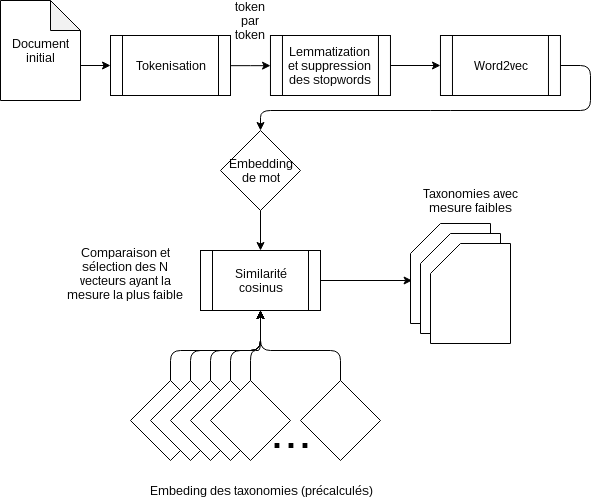
\includegraphics[width=0.8\textwidth]{taxoSchemaFoncInit.png}
	\caption[]{Schéma fonctionnel du module d'assignement taxonomique initial}
	\label{fig:taxoInit}
\end{figure}

\subsubsection{NLP}
L'utilisation des techniques du domaine du \textit{Natural Language Processing} permettent de traiter un texte pour en extraire des informations de plus haut niveau (le sens par exemple).
Le texte à analyser et la taxonomie peuvent être traités avec des méthodes de NLP afin de les normaliser et trouver les termes taxonomiques dont le sens se rapproche le plus de ce qu'on peut trouver dans le texte.

Il existe de très nombreuses méthodes de NLP utilisables pour cela, et nous avons choisi d'utiliser la \textit{lemmatisation} et la detection des mots d'importance.

La \textit{lemmatisation} consiste à transformer un mot en sa racine.
Par exemple `Nous sommes humains' deviendrait `nous être humain'.

La detection des mots d'importance nous permet d'enlever tous les mots de faible importance, et obtenir une phrase un peu plus propre.
Par exemple, `Délégation de signature' devient `Délégation signature'.


Nous avons choisi d'utiliser la méthode Word2vec, et la méthode NLP si word2vec ne fonctionnait pas, pour déduire les taxonomies d'un document, les autres méthodes n'étant pas réalisables ou pas adaptées à notre problématique.

De plus word2vec et NLP peuvent être utilisés avec une autre taxonomie sans aucun changement du code.
Cet élément est important car l'administration utilise plusieurs taxonomies. 


\subsection{Moteur de recherche}
Le moteur de recherche est la résultante visuelle de toutes les tâches techniques précédentes effectuées.
Après une étude de l'art, nous avons retenu Elasticsearch, état de l'art de la recherche open source.

Elasticsearch est le moteur de recherche open source basé sous le logiciel Apache Lucene.
A l'aide d'un fichier JSON (JavaScript Object Notation) contenant les informations structurées extraites des documents, il indexe les documents via des requêtes HTTP\@.
Plusieurs sociétés, telles que Uber, Stack Overflow ou Udemy se basent sur ce système pour la recherche de produits/documents sur leur site. 
Cette approche nous permet de nous concentrer sur l'extraction des données plutôt que les problématiques d'indexations par score des documents.

\begin{figure}[h!]
  \centering
  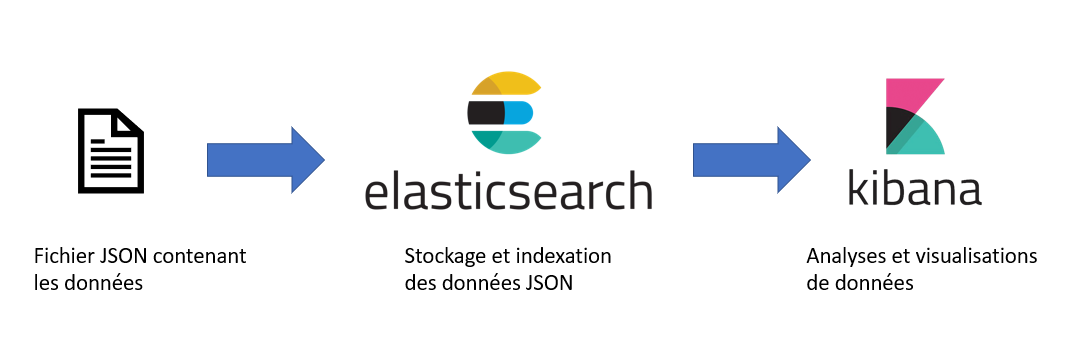
\includegraphics[width=0.8\textwidth]{ArchitectureElasticsearchKibana.PNG}
	\caption[]{Architecture Elasticsearch Kibana}
	\label{}
\end{figure}



\subsection{Interface du moteur de recherche}
Elasticsearch à lui tout seul ne suffit pas pour visualiser les données.
Comme mentionné précédemment, c'est à l’aide des requêtes HTTP que l’on peut effectuer une recherche.
Nous pouvons cependant utiliser des outils de visualisation compatibles avec Elasticsearch.

\subsubsection{Kibana}
Kibana est un greffon d'analyse de données pour ElasticSearch.

Il fournit plusieurs fonctions de visualisations qui permettent aux utilisateurs de créer des représentations visuelles (diagrammes barres/ligne, nuages de points, \ldots) pour représenter les informations de recherche Elasticsearch.

\begin{figure}[h!]
  \centering
  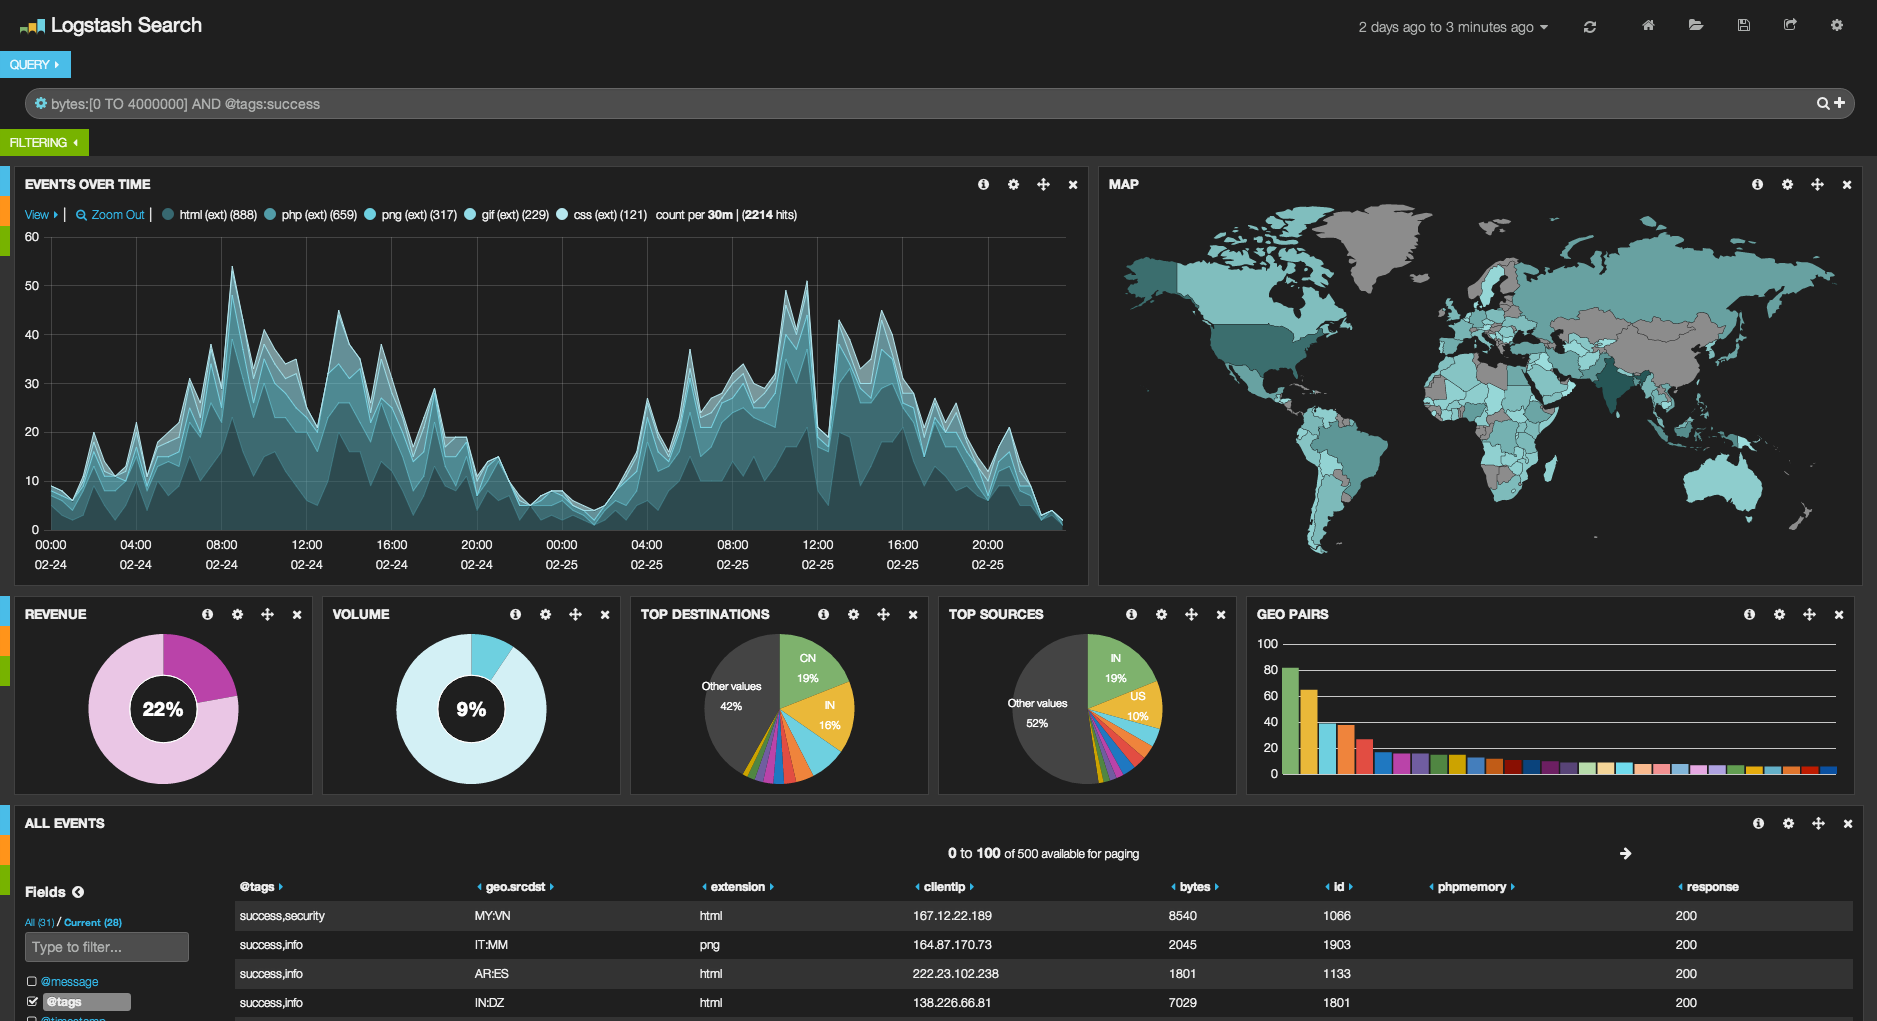
\includegraphics[width=0.8\textwidth]{visualisationKibana.png}
	\caption[]{Exemple de visualisation des données JSON sur Kibana}
	\label{}
\end{figure}
Même si pour un POC, cela est présentable, Kibana est loin d’être ergonomique.

Le couple Elasticsearch/Kibana permet de construire un moteur de recherche basique présentant une visualisation technique des données.
Cependant, cette approche est très orientée analyse de données, et il ne faut pas qu'une contrainte du PoC est qu'il doit être \textit{user-friendly}.

Premièrement, l'utilisateur doit spécifier son champ de recherche en écrivant fields.champ afin d’effectuer une recherche.
Sachant que l'utilisation du moteur de recherche sera effectuée par plusieurs personnes de la préfecture non qualifié techniquement, il serait préférable qu'il soit simple d'utilisation.

De plus, les fonctionnalités de Kibana sont orientées analyse de données, ce qui n'est pas notre sujet principal.

\begin{itemize}
    \item Avantages 
        \begin{itemize}
            \item Indexation directe avec Elasticsearch
            \item Visualisation des données
        \end{itemize}
    \item Inconvénient 
        \begin{itemize}
        \item Orienté analyse de données
        \end{itemize}
\end{itemize}


\subsubsection{Reactivesearch/Appbase.io}
Reactivesearch comme son nom l'indique se compose de React associé à Elasticsearch.
React aussi appelé React.js ou ReactJS est une bibliothèque JavaScript développée par Facebook en 2013.

Le but principal de cette bibliothèque est de faciliter la création d'application web mono page, en mettant des composants à disposition de l'utilisateur pour générer une page (ou portion) HTML lors d'un changement d'état.

Plusieurs sociétés telles que Facebook, Netflix, Yahoo ou WhatsApp l'utilisent.
Son avantage est sa facilité d'utilisation et de développement: certains outils graphiques permettent de créer une page web en moins d'une heure.

Utiliser le site \href{https://appbase.io/}{appbase.io} pour programmer avec Reactivesearch est également très intuitif.
Ce site permet d'importer des données au format JSON et d'obtenir directement un template de site mono page\@.

De plus, Reactivesearch est relié à des outils d'analyse et de statistiques des recherches effectuées par les utilisateurs.
Appbase se compose d'un \textit{Daily search volume} listant l'historique des recherches effectuées sur notre page Reactivesearch. 

Lors de l'import des données JSON, un ID personnel est envoyé, et permet aux possesseurs de l'ID d'accéder au JSON en ligne.
De cette manière, seule les personnes en possession de l'ID peuvent accéder et développer une page web avec les données du JSON importée. 

\begin{figure}[h!]
  \centering
  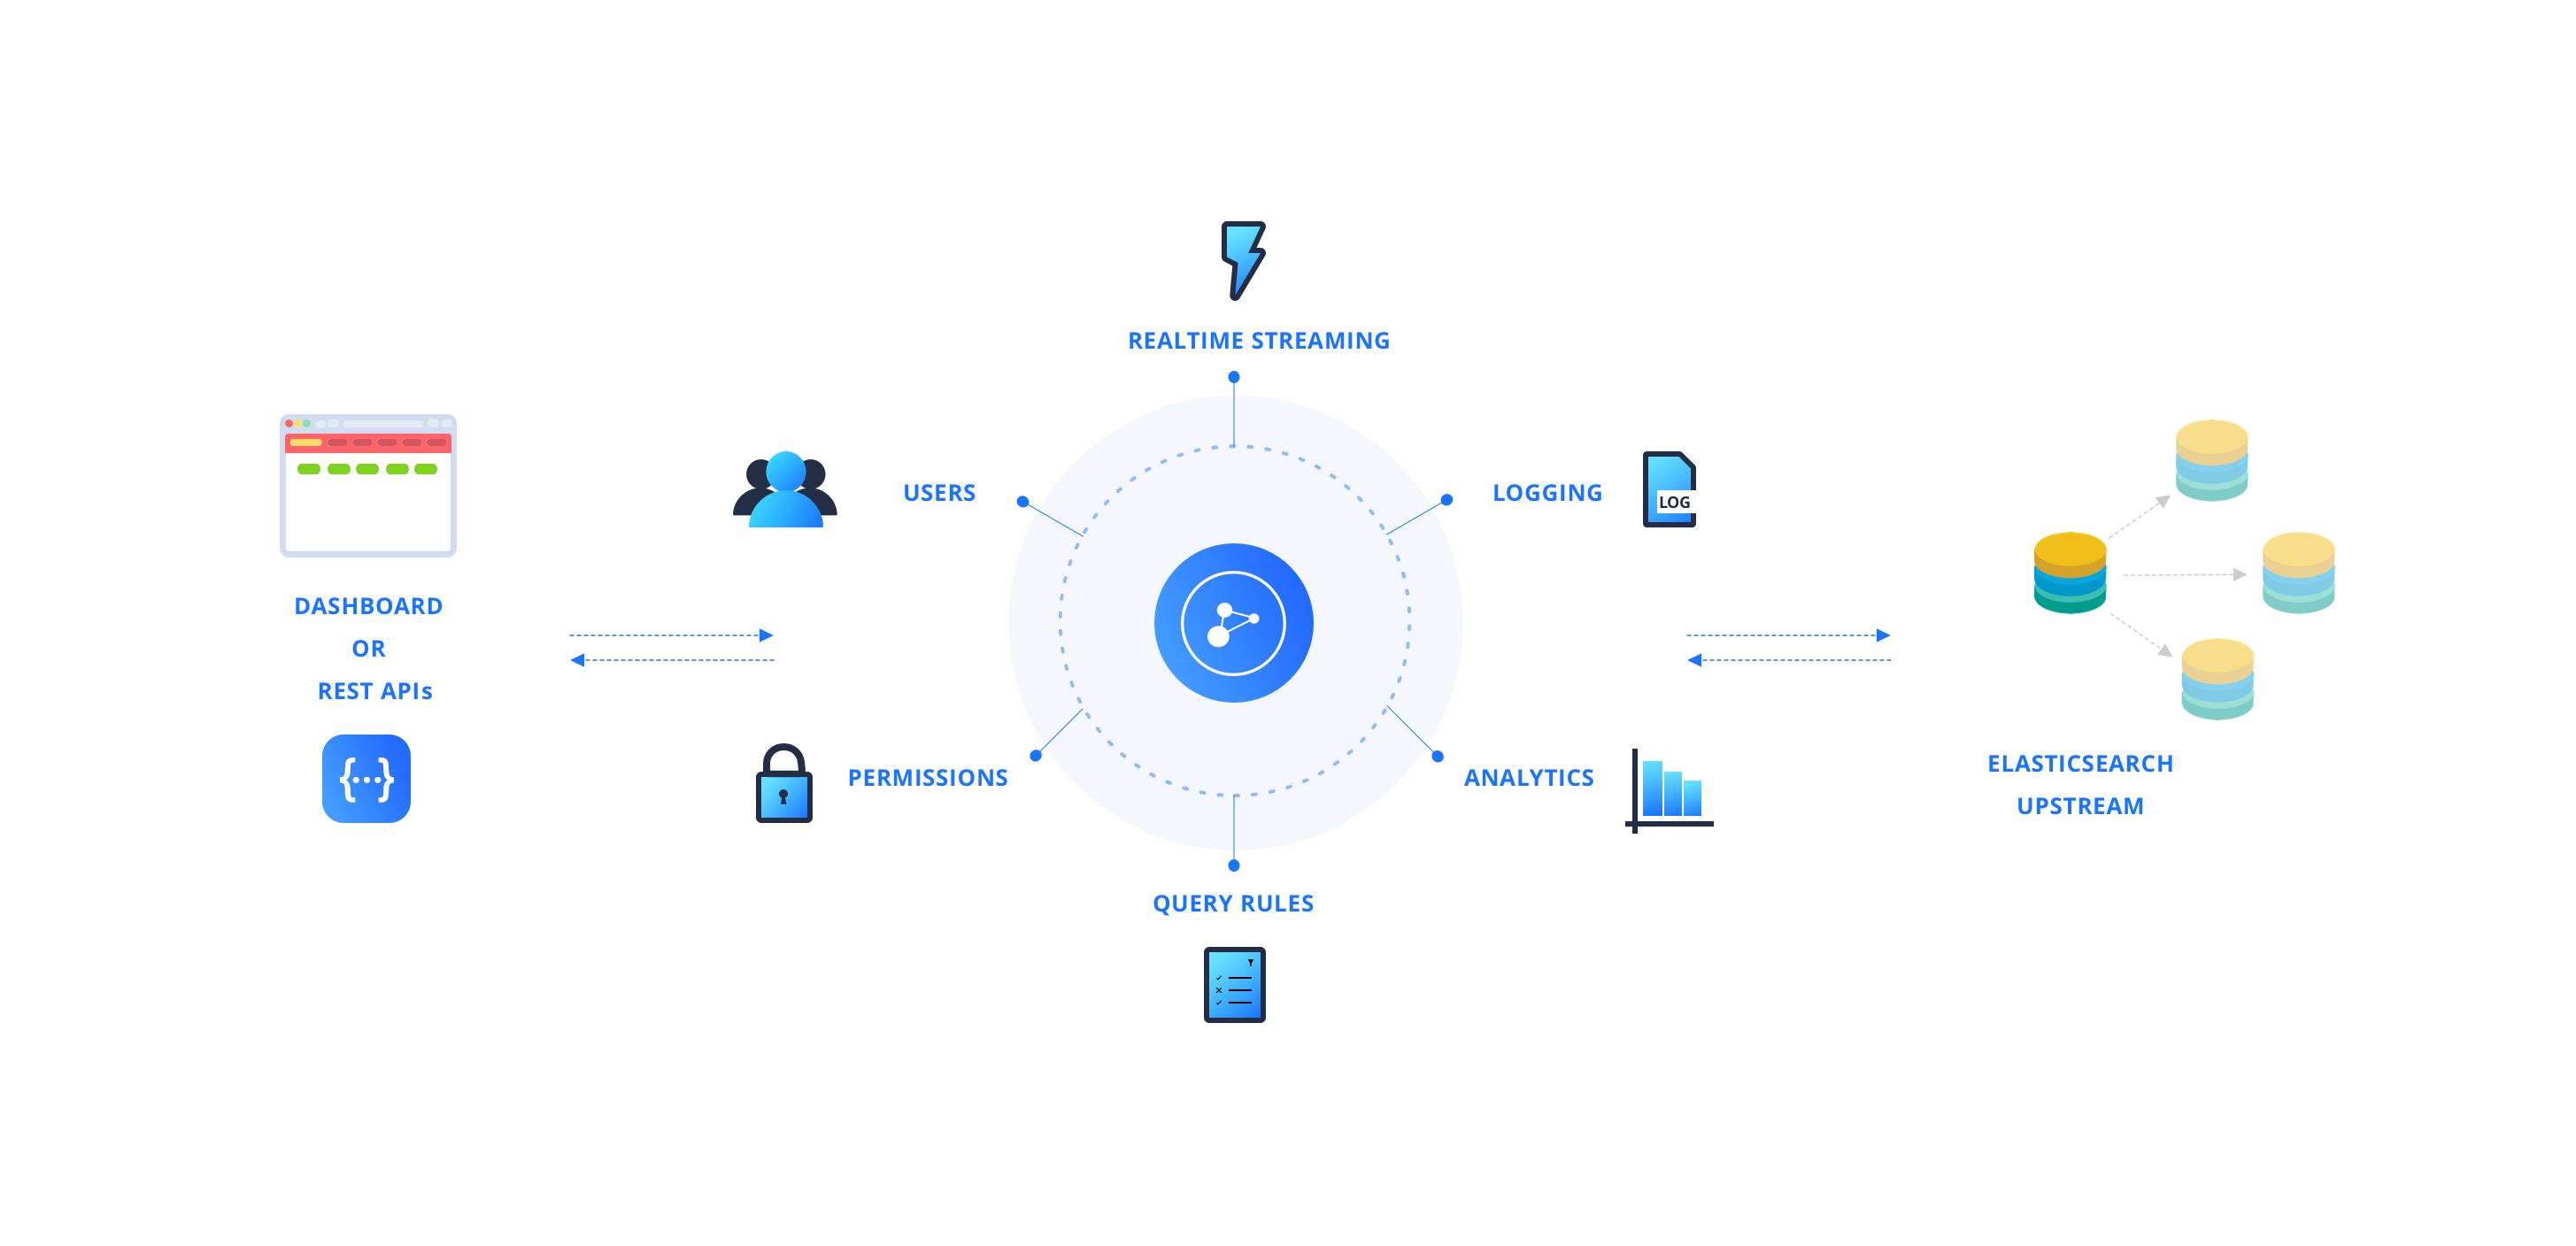
\includegraphics[width=\textwidth]{images/ArchitectureElasticsearchAppbase.png}
	\caption[]{Architecture Appbase.io et Elasticsearch}
	\label{archi_appbase}
\end{figure}

\newpage
\begin{itemize}
    \item Avantages 
        \begin{itemize}
            \item Indexation avec Elasticsearch
	    \item Simple d'implémentation
	    \item Analyse des historiques de recherche
	    \item Mufti plateformes car en ligne
        \end{itemize}
    \item Inconvénients 
        \begin{itemize}
	    \item Monopage (pas gênant pour notre application)
	    \item Sécurité relative de l’accès aux données avec les credentials
        \end{itemize}
\end{itemize}

Cette approche d’implémentation répond aux inconvénients de la visualisation avec Kibana.
Les données stockées et récupérées par notre projet ne sont pas privées, ce qui ne rend pas l'utilisation des credentials contraignantes.

Nous avons choisis donc choisi d'utiliser Reactivesearch pour les nombreux avantages par rapport à Kibana. 


